\documentclass[thesis=B,czech,hidelinks]{thesis}[2012/06/26]

\usepackage[utf8]{inputenc}

\usepackage{amsthm}
\usepackage{dirtree}
\usepackage{graphicx}
\usepackage{listings}
\usepackage{verbatim}

\department{Katedra softwarového inženýrství}
\title{Implementace důkazového systému pro výrokovou logiku}
\authorGN{Jan}
\authorFN{Švajcr}
\authorWithDegrees{Jan Švajcr}
\supervisor{Mgr. Jan Starý, Ph.D.}
\acknowledgements{Děkuji svému vedoucímu práce Mgr. Janu Starému, Ph.D. za přívětivost a pomoc, své rodině za podporu a zázemí a své milované za lásku a věrnost.}
\abstractCS{Cílem této práce je vypracovat terminálovou aplikaci implementující prostředí důkazového systému výrokové logiky. Jeho hlavní funkcionalitou je syntaktická analýza textového vstupu v~podobě posloupnosti výrokových formulí a ověření, zdali je tato posloupnost korektním výrokovým důkazem. Software je implementován v~jazyce C++ a je podporován prostředím UNIX. Součástí práce je dokumentace zdrojového kódu a uživatelská příručka v~podobě standardní manuálové stránky.}
\abstractEN{The goal of this thesis is to create a command line application implementing the proof system environment of the propositional logic. It's main functionality is parsing a textual input representing a sequence of propositional formulas and verifying this sequence as a proof. The software is implemented in the C++ language and is supported by UNIX environment. Code documentation and a standard manual page as a user manual are also included.}
\placeForDeclarationOfAuthenticity{V~Praze}
\declarationOfAuthenticityOption{2}
\keywordsCS{Výroková logika, Důkazový systém, Parsing, C++.}
\keywordsEN{Propositional logic, Proof system, Parsing, C++.}

%
%
%

\begin{document}

\theoremstyle{definition}
\newtheorem{exm}{Příklad}
\newtheorem{dfn}{Definice}

%
%
%

\begin{introduction}
Logika je formální věda zkoumající část lidského myšlení. Jejím předmětem je správné vyvozování důsledků z~předpokladů, jejichž volbu, pravdivost nebo snad smysl blíže nezkoumáme. Nečiníme tak nejen proto, že naše vyvození je správné i v~případě, kdy předpoklady správné nejsou, ale i proto, že to této disciplíně ani nepřísluší. Matematická logika toto usuzování formalizuje, čímž nás oprošťuje od psychologického aspektu. Dává tak vzniknout postupům, které lze kdykoliv opakovaně aplikovat. Příkladem takového postupu je ověřování správnosti našeho usuzování, tzv. důkazu. To je dokonce natolik mechanické, že jej můžeme svěřit strojovému zpracování\cite{sochor}. Právě tento aspekt výrokové logiky byl podnětem pro vznik této práce, která formalismus výrokové logiky implementuje počítačovým programem. Konkrétně implementuje principy Hilbertova systému. Ústřední kapitolou výrokového počtu, o~kterou se budeme v~rámci teoretické přípravy zajímat zejména, je \emph{dokazatelnost}.

Ještě předtím než se ponoříme do problematiky implementace, je třeba analyzovat vlastnosti příslušné oblasti výrokového počtu. V~první kapitole proto vysvětlíme klíčové pojmy výrokové logiky, které nás budou provázet životním cyklem projektu a budou tak pro nás nutnou znalostí. Pokračovat budeme kapitolou, ve které upřesníme zadání projektu a vymezíme požadavky na implementaci. Následuje kapitola, ve které položíme základy pro vlastní implementaci. Budeme se zde věnovat rozkladu systému na menší celky a návrhu jejich řešení. K~softwarové realizaci přejdeme v~navazující kapitole zabývající se technickými detaily samotné implementace. Nastíníme zde význam datových struktur a popíšeme klíčové algoritmy. Předposlední kapitola se věnuje testování. Budeme se zde snažit maximálně pokrýt rizikové oblasti, které mohou ohrozit stabilitu aplikace. Práci zakončíme krátkým zamyšlením nad jejím možným pokračováním a prodiskutujeme její rozšířitelné stránky.
\end{introduction}

%
%
%

\chapter{Formální kontext}

V~úvodní kapitole se seznámíme s~několika základními pojmy výrokového počtu a zavedeme terminologii užitou v tomto textu, abychom na ni mohli čtenáře později odkázat. Tato část slouží jako teoretický základ celé práce. Čtenář znalý výrokové logiky ji může vynechat.

\section{Výrok}

Nejprve zavedeme elementární pojem \emph{výrok}.

Výrok je takové tvrzení, o kterém má smysl uvažovat, zdali je pravdivé či nikoliv. Výrokům tedy přiřazujeme \emph{pravdivostní hodnoty} pravda (true) nebo nepravda (false)\cite{sochor}.

\begin{exm}
např. věta \uv{Dnes je hezký den} je výrok. Je na čtenáři, aby rozhodl o pravdivosti tohoto výroku. Jiný čtenář by mohl případně rozhodnout opačně.
\end{exm}
 
V této práci se však pravdivostním ohodnocením výroků ani jejich významem nebudeme zabývat.

Výroková logika od vnitřní struktury výroků abstrahuje v pojmu \emph{elementárního výroku}, ze kterých buduje \emph{výrokové formule} pomocí \emph{logických operací}. Jednotlivé elementární výroky značíme velkými písmeny latinky: $A, B, C, \ldots$

\section{Logické operace}

Logické operace dělíme na unární a binární podle jejich arity\footnote{Arita -- počet operandů operace potřebných k~jejímu provedení.}. Symbolicky je reprezentují příslušné logické spojky následovně:

\begin{itemize}
	\item Unární
	\begin{description}
		\item[Negace] $\neg$
	\end{description}
	\item Binární
	\begin{description}
		\item[Konjunkce] $\wedge$
		\item[Disjunkce] $\vee$
		\item[Implikace] $\Rightarrow$
		\item[Ekvivalence] $\Leftrightarrow$
	\end{description}
\end{itemize}

Každá operace specificky určuje pravdivostní hodnotu složeného výroku v~závislosti na ohodnocení výroků, které pojí. Analogii s logickými operátory lze vidět v operátorech aritmetických. Význam uvedených operací nebudeme zkoumat, protože není pro účely této práce podstatný. Zkoumáme pouze výrokové formule a jejich posloupnosti jako čistě syntaktické objekty.

\section{Formule}

Ústředním pojmem pro tuto práci je \emph{formule}.

\begin{dfn}
\label{dfn:formula}
Ve výrokové logice definujeme formuli takto:

\begin{enumerate}
	\item Každá elementární formule je formulí.
	\item Vznikne-li $\alpha$ unární logickou operací z~formule $\beta$ nebo binární logickou operací z~formulí $\beta$ a $\gamma$ , je $\alpha$ také formulí.
	\item Každá formule vznikne konečnou aplikací předchozích pravidel\cite{sochor}.
\end{enumerate}
\end{dfn}

Jednotlivé formule značíme malými písmeny řecké abecedy: $\alpha , \beta , \gamma , \ldots$

\begin{exm}
Pro ilustraci uvažujme dvě následující formule $\alpha, \beta$:
\begin{itemize}
	\item $\alpha = A$
	\item $\beta = \neg (A \vee B)$
\end{itemize}
Formule $\alpha$ je elementární formulí, kdežto formule $\beta$ je složená z~několika formulí. Pro názornost popíšeme výstavbu formule $\beta$ podle předchozí definice.
\begin{enumerate}
	\item $A$ a $B$ jsou elementární formule (výroky).
	\item Formule $A, B$ pojí operace disjunkce do podoby složeného výroku $A \vee B$.
	\item Na dosavadní formuli aplikujeme unární operaci negace, čímž vznikne formule $\beta = \neg (A \vee B)$.
\end{enumerate}
\end{exm}

\subsection{Notace}

Nyní popíšeme několik způsobů zápisu výrokových formulí.

Výrokové formule lze zapisovat ve třech, sémanticky ekvivalentních, notacích: \emph{prefixní}, \emph{infixní} a \emph{postfixní}. Tyto notace se liší pouze pořadím výpisu logické spojky ve složených výrocích.

\begin{exm}
Následující jsou různé zápisy téže formule:
\begin{description}
	\item[prefixní] $\neg \vee \alpha \: \beta$
	\item[infixní] $\neg (\alpha \vee \beta)$
	\item[postfixní] $\alpha \: \beta \vee \neg$
\end{description}
\end{exm}

Všimněme si, že v~případě prefixní a postfixní notace je přednost operací určena jednoznačně na rozdíl od notace infixní, která vyžaduje užití závorek. Je třeba brát na vědomí, že s~rostoucí složitostí formule je pro nás čím dál obtížnější udržet pozornost nad její strukturou. Protože infixní zápis je našemu vnímání nejpřirozenější, budeme jej v~této práci používat i nadále.

\section{Důkazový systém}
\label{sec:proof_system}

\emph{Důkazový systém} výrokové logiky rozhoduje o \emph{dokazatelnosti} výrokových formulí. Každý takový systém je tvořen dvěma součástmi:

\begin{itemize}
	\item Množinou axiomů
	\item Množinou odvozovacích pravidel
\end{itemize}

\emph{Axiomy} jsou schemata výrokových formulí jistého tvaru. Každou formuli ve tvaru popsaném axiomem nazýváme \emph{instancí} tohoto axiomu. Instancí axiomů je tedy nekonečně mnoho, stejně jako výrokových formulí.

Odvozovací pravidla popisují způsoby, jakými lze z daných výrokových formulí odvozovat formule další.

\subsection{Hilbertův systém}

\emph{Hilbertův systém} je důkazový systém klasické výrokové logiky. Za účelem úspornosti jazyka se omezuje pouze na dvě logické spojky: negaci a implikaci. Tyto dvě spojky tvoří tzv. \emph{minimální univerzální množinu}, proto všechny ostatní spojky můžeme vyjádřit těmito a touto redukcí neomezujeme vyjadřovací možnosti jazyka\cite{stary}. Způsob, jakým lze vyjadřovat jedny spojky pomocí druhých, zkoumat nebudeme.

Axiomem Hilbertova systému je každá formule některého z následujících syntaktických tvarů:

\begin{description}
	\item[A1] $( \varphi \Rightarrow ( \psi \Rightarrow \varphi ))$
	\item[A2] $(( \varphi \Rightarrow ( \psi \Rightarrow \chi )) \Rightarrow (( \varphi \Rightarrow \psi ) \Rightarrow ( \varphi \Rightarrow \chi )))$
	\item[A3] $(( \neg \varphi \Rightarrow \neg \psi ) \Rightarrow (( \neg \varphi \Rightarrow \psi ) \Rightarrow \varphi ))$
\end{description}

Množina odvozovacích pravidel obsahuje jediný prvek, pravidlo \emph{modus ponens}, které je zavedeno následovně:

\begin{dfn}
Z formulí $\varphi$ a $\varphi \Rightarrow \psi$ odvoď formuli $\psi$.
\end{dfn}

V~této práci se nadále budeme zabývat výhradně tímto axiomatickým systémem.

\subsection{Důkaz}

Nyní zavedeme klíčový pojem \emph{důkaz}.

\begin{dfn}
Buď $\varphi$ výroková formule. Řekneme, že konečná posloupnost výrokových formulí $\varphi_1 , \ldots, \varphi_n$ je důkazem formule $\varphi$, pokud $\varphi_n$ je formule $\varphi$, a každá formule $\varphi_i$ z~této posloupnosti je buďto instancí některého axiomu, nebo je z~některých předchozích $\varphi_j, \ldots , \varphi_k$, kde $j, \ldots , k < i$, odvozena odvozovacím pravidlem. Pokud existuje důkaz formule $\varphi$, řekneme, že je tato formule je dokazatelná ve výrokové logice, a píšeme $\vdash \varphi$\cite{stary}.
\end{dfn}

Každý důkaz tedy nutně začíná axiomem a triviálně každá instance axiomu je dokazatelnou formulí.

Pro nás klíčová je skutečnost, že důkaz vychází z~konečně mnoha daných předpokladů, postupuje dle konečně mnoha daných pravidel a je v~každém kroku ověřitelný, což lze provést i mechanicky\cite{stary}. Na druhou stranu nám to nedává žádný návod, jak případně důkaz dané formule nalézt. Ostatně tato problematika již přesahuje rozsah této práce.

\begin{exm}
\label{exm:proof_a>a}
Pro ilustraci předvedeme důkaz formule $\varphi \Rightarrow \varphi$ v Hilbertově systému.
\begin{description}
	\item[axiom 1] $(\varphi \Rightarrow ((\varphi \Rightarrow \varphi) \Rightarrow \varphi))$
	\item[axiom 2] $((\varphi \Rightarrow ((\varphi \Rightarrow \varphi) \Rightarrow \varphi)) \Rightarrow ((\varphi \Rightarrow (\varphi \Rightarrow \varphi)) \Rightarrow (\varphi \Rightarrow \varphi)))$
	\item[modus ponens, formule 1 a 2] $((\varphi \Rightarrow (\varphi \Rightarrow \varphi)) \Rightarrow (\varphi \Rightarrow \varphi))$
	\item[axiom 1] $(\varphi \Rightarrow (\varphi \Rightarrow \varphi))$
	\item[modus ponens, formule 4 a 3] $(\varphi \Rightarrow \varphi)$
\end{description}
\end{exm}

\subsubsection{Důkaz z~předpokladů}
\label{sec:proof_theory}

Důkaz lze zobecnit na tzv. \emph{důkaz z~předpokladů} rozšířením stávající definice důkazu. Navíc zavedeme množinu \emph{předpokladů} $T$, tj. formulí, ze kterých v~rámci důkazu vycházíme. Zobecnění spočívá v~tom, že kromě axiomů jako členy důkazu obdobně připouštíme i formule z množiny předpokladů. Předpoklad je tedy formule, kterou, ačkoliv není axiomem, elementárně považujeme za dokazatelnou. Existuje-li důkaz formule $\varphi$ z předpokladů $T$, píšeme $T \vdash \varphi$.

\subsubsection{Optimalizace důkazů}

Protože se v této práci také zabýváme optimalizací, resp. minimalizací, důkazů, definujeme nyní důkaz, který nazveme \emph{optimálním}.

\begin{dfn}
\label{dfn:optimal_proof}
Buď $\varphi_1, \ldots, \varphi_n$ posloupnost formulí tvořící důkaz formule $\varphi_n$. Důkaz nazveme optimálním, pokud každá formule $\varphi_i$, kde $i < n$, je nezbytná k důkazu formule $\varphi_n$, tj. je jejím přímým či nepřímým svědkem za použití odvozovacích pravidel.
\end{dfn}

Takový důkaz tedy neobsahuje zbytečné vnořené důkazy a neobsahuje ani duplicitní formule, protože, pokud nějaká formule $\varphi_i$ vyplývá z~nějakých předchozích formulí pomocí odvozovacího pravidla, pak stejným způsobem vyplývá i z~každých jejich předchozích, speciálně z~prvních, výskytů.

Z optimálního důkazu se tedy již nedá odstranit žádná formule, důkaz by jinak přestal být korektním. Neznamená to však, že neexistuje jiný důkaz téže formule, který by byl např. úspornější. Hledání takového důkazu však opět přesahuje rozsah této práce.

%
%
%

\chapter{Vymezení požadavků}

Na základě oficiálního zadání této práce, kterým začíná tento text, vymezíme v~této kapitole požadavky na implementovaný software. Tyto požadavky kategorizujeme na \emph{funkční} a \emph{nefunkční}.

Funkční požadavky definují cíle, kterých má projekt dosáhnout. V~našem případě se jedná o~funkcionalitu námi implementovaného software. Na základě funkčních požadavků lze navrhnout metody testování a ověřit úspěšné splnění zadání na konci projektu.

Mezi nefunkční požadavky řadíme náležitosti, které popisují způsob, jakým máme provést implementaci. Některé z~nich jsou součástí zadání, některé si pro úplnost zadání stanovíme sami. Nefunkční požadavky jsou omezení, ze kterých vycházíme, a nejsou předmětem testování.

\section{Funkční požadavky}

Úkolem je vypracovat aplikaci \emph{pl} (propositional logic), která primárně dokáže rozhodnout, zdali je daná posloupnost výrokových formulí korektním formálním důkazem Hilbertova systému. Požadavkem nad rámec zadání je optimalizace těchto důkazů. Elementární funkcionalitou programu je syntaktická analýza vstupních formulí a jejich případný výpis ve zvolené alternativní notaci a jazyce. Nekorektní vstup program správně detekuje a případně jeho nekorektnost podrobně hlásí.

Aplikaci je třeba náležitě otestovat a metody užité při testování zdokumentovat. Dále je třeba vytvořit dokumentaci zdrojového kódu a uživatelskou příručku k aplikaci.

\section{Nefunkční požadavky}

\subsection{Aplikace}

Aplikace bude podporována na platformách systému UNIX a implementována v~jazyce C++. Její obsluha bude možná přes systémový terminál, tedy nebude disponovat grafickým uživatelským rozhraním. To nepředstavuje žádné podstatné omezení funkcionality, neboť pracujeme pouze s textovým vstupem. Veškerá funkcionalita aplikace bude dostupná standardně pomocí přepínačů příkazové řádky. Vstupní data budou aplikaci předávána buďto na standardním vstupu, anebo v textovém souboru. Návratová hodnota programu bude signalizovat úspěšnost výsledku.

\subsection{Vstup}

Aplikace čte buď ze standardního vstupu anebo ze souboru textový ASCII vstup v~podobě posloupnosti řádek obsahujících výrokové formule zapsané ve stanoveném jazyce. Podporován je prefixní, infixní i postfixní zápis formulí. Vstup nevyhovující stanovené formě je považován za nekorektní a je odmítnut.

\subsection{Výstup}

Forma výstupu závisí na zvolené funkcionalitě, ke které je program nakonfigurován při spuštění. Podporován je výpis formulí v~prefixní, infixní i postfixní notaci. Výstupní jazyk formulí může mít podobu ASCII znaků, přirozeného jazyka nebo jazyka \LaTeX. Výstupem programu může být v~určitých případech chybové hlášení o nekorektním vstupu.

\subsection{Dokumentace}

Programátorská dokumentace bude dostupná v~podobě HTML stránek za použití nástroje \emph{Doxygen}, který takovou dokumentaci generuje. Zdrojový kód programu proto opatříme komentáři speciálního stylu, který tento nástroj vyžaduje.

\subsection{Příručka}

Uživatelskou příručku realizujeme v~podobě standardní manuálové stránky operačních systémů UNIX. Tato stránka bude po instalaci přístupná standardně pomocí příkazu \texttt{man pl}.

%
%
%

\chapter{Analýza a návrh}

\section{Technický kontext}

V této části popíšeme technologie, které jsme pro implementaci stanovili nefunkčními požadavky, a odůvodníme jejich užití.

\subsection{C++}

Programovací jazyk C++ je rozšířením jazyka C. Vybrali jsme jej zejména proto, že podporuje objektově-orientované paradigma, kterého se budeme držet. Přednosti tohoto programovacího stylu nám usnadní nejen implementaci, ale i návrh. Přitom také dbáme na přenositelnost a rozšiřitelnost aplikace, jak požaduje zadání.

Pro jazyk C++ existuje velké množství standardních knihoven, které nabízejí běžné funkce či běžné datové typy. Jejich užití vede k úspoře zdrojového kódu a menší míře zanesených chyb. Při implementaci budeme maximálně využívat těchto standardních knihoven. Naopak, nebudeme využívat prostředky třetích stran. Zejména využijeme knihovny STL obsahující šablony základních kontejnerů.

\subsubsection{C++11}

C++11 je jedním z posledních standardů jazyka C++. Vybrali jsme jej především z důvodu úspory kódu, což umožňují některé konstrukty, které tento standard zavedl, zejména např. alternativní zápis cyklu \texttt{for}, který abstrahuje od iterátorů při procházení kontejnerů\cite{cpp}.

\subsection{Make}

Nástroj \texttt{make} slouží k zjednodušení sestavování programů. Jeho předností je zejména schopnost na základě časové známky určit, které součásti programu jsou třeba zkompilovat v případě změny zdrojového kódu. K řízení sestavení tento nástroj využívá konfiguračního souboru \texttt{Makefile}. Ten má předepsanou strukturu a obsahuje definice pravidel, tzv. \emph{cílů}, které mají svůj název a konkrétní účel. Cíl je definován posloupností příkazů pro \texttt{shell}, které jsou provedeny při jeho volání. Každý cíl může navíc obsahovat \emph{závislosti}. Závislost je další cíl, který je volán přednostně. Speciálními (konečnými) cíly bývá kompilace konkrétního zdrojového souboru\cite{gmake}.

My použijeme nástroj GNU \texttt{make}, který je jednou z implementací klasického \texttt{make} rozšířenou o pokročilé funkce. Z nich konkrétně využijeme např. \emph{pattern rules}, \emph{wildcard characters} či \emph{string functions}\cite{gmake}

\subsection{Doxygen}

Doxygen je nástroj pro automatickou tvorbu dokumentace zdrojového kódu. Umožňuje dokumentovat kód mnohých populárních programovacích jazyků, zejména C++. Podporuje různé formy výstupu, přičemž my zvolíme dokumentaci v podobě HTML stránek. Text dokumentace tento nástroj čerpá přímo ze souborů zdrojového kódu prostřednictvím speciálních komentářů. To zajišťuje neustálou konzistenci mezi dokumentací a zdrojovým kódem. Tento nástroj funguje i v případě nezdokumentovaného kódu, kdy alespoň podá základní přehled o prvcích zdrojového kódu. V neposlední řadě je schopen vizualizovat relace mezi elementy v podobě diagramů jako je např. diagram tříd\cite{doxygen}.

My budeme dokumentaci zapisovat především do hlavičkových souborů \texttt{.hpp}, aby nepřekážela v implementaci.

\subsection{Mdoc}

Manuálové stránky systému UNIX lze psát ve speciálním značkovacím jazyce. Takový jazyk je ve skutečnosti balíček maker pro jazyk \emph{troff}. Troff pochází ze 70. let a podobně jako např. \LaTeX slouží k~sazbě textu. Jazyk zpracovává stejnojmenný textový procesor, který podporuje právě zmíněné balíčky maker pro tento jazyk. Jednotlivá makra, podobně jako např. značky jazyka HTML, formátují daný obsah do požadované podoby\cite{troff}. Běžné manuálové stránky užívají balíček maker \texttt{man}. My však zvolíme sofistikovanější balíček \texttt{mdoc}, který narozdíl od \texttt{man} disponuje sémantickou koncepcí maker. Záznam o~tomto balíčku nalezneme mimo jiné v~sekci \emph{mdoc(7)} manuálových stránek\cite{mdoc}.

\section{Analýza}

\subsection{Případy užití}
\label{sec:use_cases}

Na základě funkčních požadavků nastíníme možné případy užití aplikace \ref{fig:use_cases}.

\begin{figure}
\centering
\caption{Diagram případů užití}
\label{fig:use_cases}
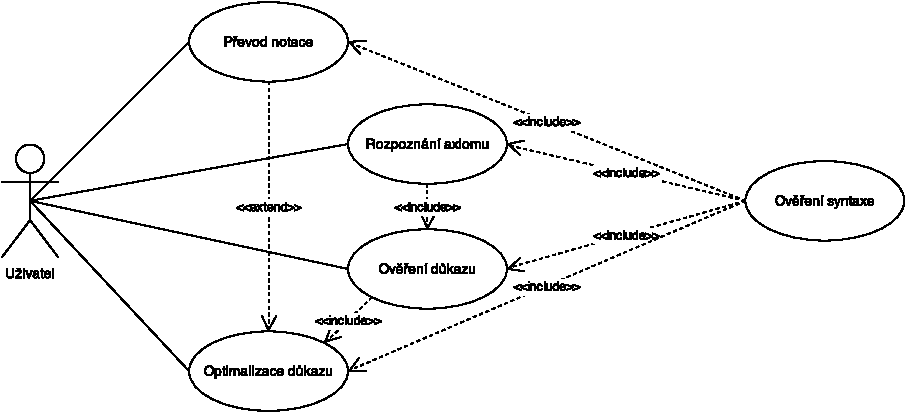
\includegraphics{diagrams/use_cases}
\end{figure}

\subsubsection{Převod notace}

Elementární funkcionalitou aplikace je převod formulí dané notace do notace vybrané. Zároveň je tato funkcionalita vhodná i pro kontrolu syntaktického zápisu formulí. Forma logických spojek výstupu je dostupná v podobě znaků ASCII (stejně jako vstup), v přirozeném jazyce nebo v jazyce \TeX.

\subsubsection{Rozpoznání axiomu}

Protože součástí ověření důkazu je rozpoznání axiomů, nabídneme tuto funkci také samostatně. Každá formule vstupní posloupnosti je potom ověřována jako axiom a na výstupu je případně uváděn jeho typ.

\subsubsection{Ověření důkazu}

Tato funkcionalita je hlavním cílem této práce. Na vstupní posloupnost formulí je nahlíženo jako na posloupnost členů důkazu, přičemž aplikace ověří, zdali je důkaz korektním. Je možné ověřovat i důkaz z předpokladů. Tehdy je prvních $n$ vstupních formulí považováno za prvky teorie, pak následují formule vlastního důkazu. Výstupem aplikace jsou podrobnosti o dokazatelnosti, popř. nedokazatelnosti každého členu důkazu.

\subsubsection{Optimalizace důkazu}

Důkaz (z předpokladů) je nejprve ověřen stejně jako v předchozím případě. Následně, pokud je to možné, je optimalizován do nejúspornější možné podoby \ref{def:optimal_proof}. Výstupem je důkaz téže formule právě v této podobě.

\section{Návrh}

\subsection{Forma vstupu}

Textový vstup aplikace \texttt{pl} se skládá z posloupnosti formulí, přičemž každá z nich je zakončena řádkovým zalomením (\texttt{\\n}. Zápis formulí užívá znaků \texttt{A-Z} pro elementární výroky. Tím je vstup omezen na 26 různých elementárních výroků, což ovšem pro naše účely plně postačuje. Symboly \texttt{-.+>=} značí logické operátory negace, konjunkce, disjunkce, implikace a ekvivalence. Pro infixní notaci formulí navíc zavádíme symboly závorek\texttt{()} pro určování přednosti operací.

\subsection{Forma výstupu}

Kromě výstupní notace lze zvolit i jednu ze tří výstupních forem (jazyků) logických spojek. Jak jsou jednotlivé operátory zastoupeny v těchto jazycích znázorňuje tabulka \ref{tab:connectives_language}.

\begin{table}
\centering
\caption{Výstupní jazyky spojek}
\label{tab:connectives_language}
\begin{tabular}{|c||c|c|c|}\hline
Operátor & ASCII & Slovní & \TeX \tabularnewline \hline \hline
Negace & \verb|-| & \verb|not| & \verb|\neg| \tabularnewline \hline
Konjunkce & \verb|.| & \verb|and| & \verb|\wedge| \tabularnewline \hline
Disjunkce & \verb|+| & \verb|or| & \verb|\vee| \tabularnewline \hline
Implikace & \verb|>| & \verb|implies| & \verb|\Rightarrow| \tabularnewline \hline
Ekvivalence & \verb|=| & \verb|iff| & \verb|\Leftrightarrow| \tabularnewline \hline
\end{tabular}
\end{table}

\subsection{Uživatelské rozhraní}

Nefunkčním požadavkem na uživatelské rozhraní je obsluha pomocí přepínačů. V této části tedy navrhneme přepínače aplikace \texttt{pl} pokrývající veškerou funkcionalitu stanovenou v požadavcích. 

\begin{description}
	\item[-A] (axiom checker) Ověří formule vstupní posloupnosti jako axiomy.
	\item[-e] (echo) Povolí hlášení na standardním a standardním chybovém výstupu. Implicitně není produkován žádný výstup.
	\item[-f file] (input file) Použije soubor \emph{file} jako vstup namísto (implicitního) standardního vstupu.
	\item[-i syntax] (input syntax) Nastaví danou vstupní notaci \emph{syntax} formulí s hodnotami \emph{prefix}, \emph{infix} a \emph{postfix}. Implicitní hodnota je \emph{infix}.
	\item[-l language] (output language of connectives) Nastaví danou výstupní formu jazyka logických spojek. Možné hodnoty jsou: \emph{ascii}, \emph{words} a \emph{latex}. Implicitní hodnota je \emph{ascii}.
	\item[-o syntax] (output syntax) Nastaví danou výstupní notaci \emph{syntax} formulí s hodnotami \emph{prefix}, \emph{infix} a \emph{postfix}. Implicitní hodnota je \emph{infix}.
	\item[-O n] (proof optimizer) Optimalizuje důkaz ze vstupní posloupnosti formulí. Nepovinný parametr \emph{n} vyjadřuje počet formulí množiny předpokladů, které na vstupu předcházejí skutečnému důkazu. Implicitní hodnota je 0, tedy důkaz není implicitně optimalizován jako důkaz z předpokladů.
	\item[-P n] (proof checker) Ověří vstupní posloupnost formulí jako důkaz. Nepovinný parametr \emph{n} vyjadřuje počet formulí množiny předpokladů, které na vstupu předcházejí skutečnému důkazu. Implicitní hodnota je 0, tedy důkaz není implicitně ověrován jako důkaz z předpokladů.
	\item[-s] (strict) Povolí zastavení vykonávání programu při prvním výskytu nekorektního syntaktického zápisu formule. Přepínače \emph{-O} a \emph{-P} takové chování povolují automaticky, protože nemá smysl dále optimalizovat či ověřovat evidentně nekorektní důkaz.
\end{description}

\emph{Axiom checker}, \emph{proof checker} a \emph{proof optimizer} budeme dále nazývat cíly aplikace. Volba těchto cílů je nepovinná, avšak je vždy omezena na jediný.

\subsection{Manuálová stránka}

Manuálové stránky mají standardní strukturu, kterou dodržíme. Text příručky napíšeme v~angličtině a její obsah rozdělíme do příslušných standardních sekcí následovně:

\begin{description}
	\item[NAME]  Název a krátký popis aplikace.
	\item[SYNOPSIS] Výčet podporovaných přepínačů.
	\item[DESCRIPTION] Podrobný popis aplikace.
	\begin{description}
		\item[Language] Popis vstupního jazyka.
		\item[Input] Popis formy vstupu.
		\item[Output] Popis formy výstupu.
		\item[Options] Popis podporovaných přepínačů.
	\end{description}
	\item[EXIT STATUS] Popis návratových hodnot.
	\item[EXAMPLES] Vzorové příklady užití.
	\item[HISTORY] Historický kontext aplikace.
	\item[AUTHOR] Informace o~autorovi.
\end{description}

%
%
%

\chapter{Implementace}

V této kapitole popíšeme, jak ty které části zdrojového kódu implementují doposud zmíněné prvky systému.

\section{Sestavení}

Cíle v našem \texttt{Makefile} jsme rozdělili do dvou kategorií: hlavní a podpůrné. Hlavní cíle jsou určeny uživateli aplikace, podpůrné cíle jsou využívány hlavními a slouží k~rozkladu složitějšího úkonu na jednodušší celky. Abychom si proces sestavení aplikace s pomocí nástroje \texttt{make} maximálně usnadnili, nakonfigurovali jsme jej tak, abychom nemuseli do souboru \texttt{Makefile} zasahovat po každé změně zdrojových souborů (např. přejmenování souboru nebo změna závislostí na hlavičkových souborech). Nástroj \texttt{make} tedy aplikaci sestaví dynamicky, podle aktuální podoby zdrojové formy.

Námi implementované cíle mají následující účel:

\begin{description}
	\item[build] Sestaví aplikací.
	\item[clean] Odstraní veškeré výstupy.
	\item[doc] Vygeneruje dokumentaci zdrojového kódu.
	\item[test] Otestuje aplikaci.
	\item[install] Nainstaluje aplikaci do systému.
	\item[uninstall] Odinstaluje aplikaci ze systému.
\end{description}

\subsection{Cíl build}

Speciálním podpůrným cílem je navíc pravidlo definující způsob kompilace jednotlivých zdrojových souborů. Toto pravidlo je v~procesu kompilace klíčovým, protože dynamicky vyvolává kompilaci souborů s~příponou \texttt{.cpp} a my tak nemusíme pro každý zdrojový soubor \texttt{.cpp} zvlášť definovat pravidlo pro jeho kompilaci.

\subsection{Cíl clean}

\subsection{Cíl doc}

\subsection{Cíl test}

\subsection{Cíl install}

\subsection{Cíl uninstall}

\section{Hlavní program}

Hlavní program aplikace představuje funkce \texttt{main}.

Nejdříve se program pokusí inicializovat instanci třídy \texttt{Configuration}. V případě úspěchu je proveden cíl aplikace uložený v této instanci, jehož návratová hodnota je vrácena jako návratová hodnota aplikace. V případě, že se nepodaří aplikaci nakonfigurovat, je zachycena výjimka s podrobnostmi o chybě a běh aplikace končí neúspěchem.

\section{Komponenty}

\subsection{Třída Configuration}

Tato třída představuje konfiguraci aplikace. Její konstruktor pomocí funkce \texttt{getopt} z knihovny \texttt{unistd.h} zpracovává přepínače z příkazové řádky a nastavuje třídní proměnné, podle kterých je řízen průběh aplikace. Tyto proměnné jsou pak dostupné pomocí getterů.

\subsection{Třída SyntaxException}

Tato obecná třída představuje výjimku vrženou při konfiguraci aplikace v případě nesprávné syntaxe příkazové řádky. Objekt této třídy si uchovává záznam o tom, který přepínač syntaktickou chybu způsobil, a řetězec s detaily o této chybě. Metoda \texttt{getMessage} tyto informace vrací v podobě řetězce s přehledným chybovým hlášením.

Hierarchii tříd rodiny \texttt{SyntaxException} ilustruje diagram \ref{fig:syntax_exception}.

\begin{figure}
\centering
\caption{Diagram tříd rodiny SyntaxException}
\label{fig:syntax_exception}
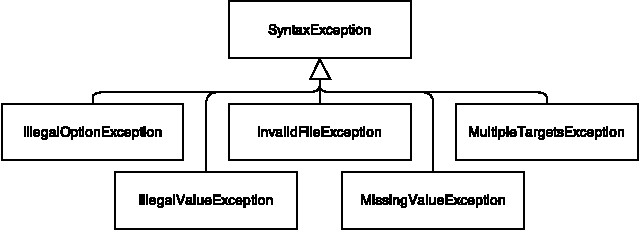
\includegraphics[width=\linewidth]{diagrams/syntax_exception}
\end{figure}

\subsubsection{Výjimka IllegalOptionException}

Výjimka tohoto typu je vržena v případě, že byl použit nepovolený přepínač.

\subsubsection{Výjimka IllegalValueException}

Výjimka tohoto typu je vržena v případě, že byla zadána nepovolená hodnota přepínače.

\subsubsection{Výjimka InvalidFileException}

Výjimka tohoto typu je vržena v případě, že byl uveden nepoužitelný vstupní soubor.

\subsubsection{Výjimka MissingValueException}

Výjimka tohoto typu je vržena v případě, že nebyla uvedena povinná hodnota přepínače.

\subsubsection{Výjimka MultipleTargetsException}

Výjimka tohoto typu je vržena v případě, že bylo nastaveno více cílů k provedení.

\subsection{Třída ExecutionTarget}

Tato třída představuje cíl aplikace. Disponuje pouze metodou \texttt{executeTarget}, která v závislosti na konfiguraci aplikace cíl provede a vrátí návratovou hodnotu aplikace.

\subsection{Třída Formula}

Výroková formule je výraz se stromovou strukturou, proto je také jako strom implementována. Tato abstraktní třída představuje uzel tohoto stromu a její návrh odpovídá definici výrokové formule \ref{dfn:formula}. Objekt této třídy obsahuje znak, který reprezentuje dílčí složenou, resp. elementární, formuli jakožto operátor, resp. výrok. Zdůrazníme, že výsledkem našeho řešení není \emph{sémantický}, ale \emph{výrazový} strom.

Hierarchii tříd rodiny \texttt{Formula} ilustruje diagram \ref{fig:formula}.

\begin{figure}
\centering
\caption{Diagram tříd rodiny Formula}
\label{fig:formula}
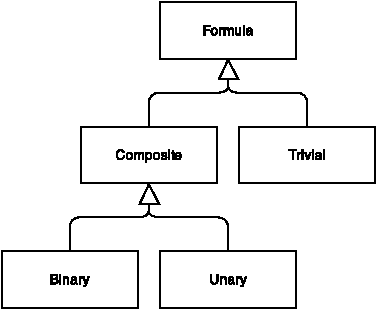
\includegraphics[width=\linewidth]{diagrams/formula}
\end{figure}

\subsubsection{Třída Trivial}

\subsubsection{Třída Composite}

\subsubsection{Třída Unary}

\subsubsection{Třída Binary}

\subsection{Parser formulí}

Parserem abstraktně nazveme tu část programu, která převádí vstup z textové do vnitřní formy. V našem případě jej reprezentují samostatné funkce \emph{parsePrefix}, \emph{parseInfix} a \emph{parsePostfix}. Každá z těchto funkcí slouží ke zpracování vstupních formulí v příslušné notaci. Syntaktická analýza postupuje po jednotlivých znacích vstupního proudu, aby mohla být přerušena již v místě případné syntaktické chyby. Funkce v případě úspěchu vrací kořen výrazového stromu formule.

Základem syntaktické analýzy je cyklus, ve kterém se okamžitě zpracovává jediný znak vstupu. Nyní částečně popíšeme algoritmy syntaktické analýzy korektního vstupu parsovacích funkcí.

\subsubsection{Funkce parsePrefix}

Prefixní parser ukládá přijaté logické operátory na zvláštní zásobník s operátory. Po přijetí elementární formule je tato nastavena jako operand zleva vrcholu zásobníku. Ve chvíli, kdy jsou operandy vrcholu zásobníku již plně obsazeny, dojde k sejmutí operátoru ze zásobníku. Tento operátor je pak nastaven jako operand zleva novému vrcholu zásobníku. To se opakuje dokud aktuální vrchol zásobníku opět nedisponuje alespoň jedním volným operandem.

\subsubsection{Funkce parseInfix}

Infixní parser ukládá přijaté logické operátory na zvláštní zásobník s operátory a elementární formule na zvláštní zásobník s formulemi. K orientaci ve struktuře formule využívá další zásobník se stavy zpracování úrovní (větví) výrazového stromu. Každá taková úroveň zpracování může mít následující stav:

\begin{description}
	\item[UNARY] Naposledy byl nastaven unární operátor. 
	\item[BLANK] Naposledy byla otevřena nová větev stromu.
	\item[FIRST\_OPERAND] Naposledy byl nastaven první operand.
	\item[BINARY] Naposledy byl nastaven binární operátor.
	\item[LAST\_OPERAND] Naposledy byl nastaven poslední operand.
\end{description}

Podle těchto stavů lze na základě jistých pravidel vždy rozhodně určit, zdali aktuálně zpracovávaný prvek neporušuje infixní syntaxi formulí. Taková pravidla popisují chování infixního parseru v závislosti na přijatém prvku a stavu zpracování aktuální větve stromu.

\subsubsection{Funkce parsePostfix}

Postfixní parser ukládá přijaté elementární formule na zvláštní zásobník s formulemi. Ve chvíli, kdy je přijat logický operátor, dojde k sejmutí příslušného počtu formulí ze zásobníku, přičemž tyto jsou zprava nastaveny jako operandy přijatého operátoru. Ten je následně uložen na zásobník.

\subsection{Třída ParseException}
\label{sec:parse_exception}

Tato obecná třída představuje výjimku vrženou při syntaktické analýze nekorektního vstupu. Objekt této třídy obsahuje řetězec s popisem příčiny syntaktické chyby. Metoda \texttt{getMessage} tuto informaci vrací v podobě řetězce s chybovým hlášením.

Hierarchii výjimek rodiny \texttt{ParseException} ilustruje diagram \ref{fig:parse_exception}.

\begin{figure}
\centering
\caption{Diagram tříd rodiny ParseException}
\label{fig:parse_exception}
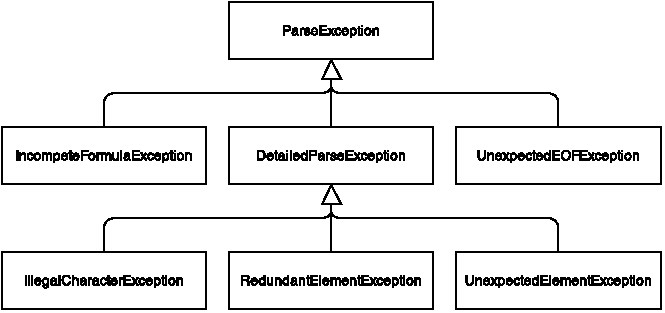
\includegraphics[width=\linewidth]{diagrams/parse_exception}
\end{figure}

\subsubsection{Výjimka IncompleteFormulaException}

Výjimka tohoto typu je vržena v případě, že vstupní formule je nekompletní.

\subsubsection{Výjimka DetailedParseException}

Tato obecná výjimka představuje syntaktickou chybu speficikovanou znakem vstupu, který chybu způsobil, a pozici tohoto znaku na řádce (kromě bílých znaků). Metoda \texttt{getMessage} je touto třídou překryta a je implementována tak, aby chybové hlášení obsahovalo tyto podrobnosti.

\subsubsection{Výjimka UnexpectedEOFException}

Výjimka tohoto typu je vržena v případě, že parser narazil na konec vstupu v místě, které nestanovuje korektní forma vstupu.

\subsubsection{Výjimka IllegalCharacterException}

Výjimka tohoto typu je vržena v případě, že vstup obsahuje nepovolený znak.

\subsubsection{Výjimka RedundantElementException}

Výjimka tohoto typu je vržena v případě, že řádek vstupu obsahuje korektní zápis formule a alespoň jeden nadbytečný prvek.

\subsubsection{Výjimka UnexpectedElementException}

Výjimka tohoto typu je vržena v případě, že infixní syntaktický zápis formule je nekorektní.

\subsection{Třída ProofSystem}

Ačkoliv tato práce implementuje Hilbertův systém jako jediný konkrétní důkazový systém, z důvodu rozšiřitelnosti jsme zavedli tuto abstraktní třídu, jejíž návrh odpovídá definici důkazového systému \ref{sec:proof_system}. Objekt této třídy obsahuje axiomy důkazového systému a implementuje metodu \texttt{isAxiom}, prostřednictvím které lze ověřit, zdali je daná formule instancí axiomu tohoto konkrétního důkazového systému. Metoda \texttt{isDeducible} slouží k odvození dané formule v rámci daného důkazu a vrací posloupnost indexů vstupních formulí, které jsou svědky odvozované formule za použití odvozovacího pravidla důkazového systému. Protože každý konkrétní důkazový systém odvozuje výrokové formule jiným způsobem, je tato metoda abstraktní.

Hierarchii tříd rodiny \texttt{ProofSystem} ilustruje diagram \ref{fig:proof_system}.

\begin{figure}
\centering
\caption{Diagram tříd rodiny ProofSystem}
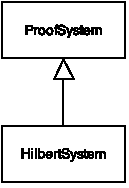
\includegraphics[width=\linewidth]{diagrams/proof_system}
\label{fig:proof_system}
\end{figure}

\subsubsection{Třída HilbertSystem}

Tato třída představuje Hilbertův systém. Je zřejmé, že je jedinou, která implementuje konkrétní důkazový systém. Pro účely odvozování formulí objekt této třídy obsahuje formuli představující implikaci pravidla modus ponens ($\varphi \Rightarrow \psi$).

Implementovaná metoda \texttt{isDeducible} odpovídá odvozování formulí pravidlem modus ponens. Její implementace spočívá v procházení jednotlivých formulí daného důkazu, přičemž na jednu z formulí je vždy nahlíženo jako na předpoklad pravidla modus ponens ($\varphi$) a na druhou jako jeho implikaci ($\varphi \Rightarrow \psi$). Daná formule $\psi$ je odvoditelná, je-li nalezena dvojice vyhovující právě tomuto tvaru.

\subsection{Třída ProofMember}

Tato třída představuje člen důkazu jako komplexní strukturu. Objekt této třídy obsahuje výrokovou formuli, která je členem důkazu, a posloupnost členů téhož důkazu, které jsou svědky tohoto členu za užití odvozovacího pravidla. V poslední řadě je zde uložena logická proměnná vyjadřující, zdali je tento člen součástí optimální podoby důkazu, jehož je členem. Tato proměnná slouží pouze algoritmu optimalizace důkazu.

\section{Manuálová stránka}

Aby manuálová stránka byla dostupná příkazem \texttt{man pl}, musí splňovat jisté náležitosti. Název souboru manuálové stránky se skládá z~názvu dokumentované aplikace, tečky a čísla příslušné manuálové sekce, v~našem případě tedy \texttt{pl.1}. Tento soubor je zabalen v archivu \texttt{.gz} a nachází se v~umístění, ve kterém příkaz \texttt{man} implicitně hledá manuálové stránky. Tato umístění jsou nastavena v~konfiguračním souboru \texttt{/etc/manpath.config} a lze je případně vypsat příkazem \texttt{manpath}. Archiv manuálové stránky je dále nutné umístit do podadresáře příslušícího dané manuálové sekci, v~našem případě do adresáře \texttt{man1}. Absolutní cesta k~naší manuálové stránce tedy může vypadat následovně: \texttt{/usr/local/man/man1/pl.1.gz}. Nakonec ještě souboru archivu nastavíme příslušné atributy dle vzoru systémových manuálových stránek, vlastník a skupina: root, práva: 0644.

Manuálovou stránku tvoří dvoupísmenná makra. Začíná-li makro na začátku řádku, předchází mu znak tečka. V~textu manuálové stránky se nesmí vyskytovat prázdný řádek.

Korektní manuálová stránka začíná následujícími makry v~dodrženém pořadí:

\begin{description}
\centering
	\item[Dd] Datum dokumentu ve formátu [měsíc den, rok].
	\item[Dt] Titulek dokumentu (velká písmena).
	\item[Os] Operační systém.
\end{description}

Naše implementace potom vypadá následovně:

\begin{verbatim}
\centering
.Dd May 10, 2014
.Dt PL 1
.Os Ubuntu Linux 14.04
\end{verbatim}

Při tvorbě manuálové stránky dále využijeme makra \texttt{Sh} pro úvod nových sekcí, případně \texttt{Ss} pro úvod sekcí druhé úrovně.

\subsection{Sekce NAME}

V~sekci \texttt{NAME} definujeme makrem \texttt{Nm} název aplikace a makrem \texttt{Nd} definujeme krátký popis účelu aplikace.

\begin{verbatim}
\centering
.Sh NAME
.Nm pl
.Nd handle formulas of propositional logic
\end{verbatim}

\subsection{Sekce SYNOPSIS}

V~sekci \texttt{SYNOPSIS} stanovíme makry \texttt{Op}, \texttt{Fl} a případně \texttt{Ar} výčet podporovaných přepínačů.

\begin{verbatim}
\centering
.Sh SYNOPSIS
.Nm
.Op Fl [přepínač] Ar [argument]
.
.
.
\end{verbatim}

\subsection{Sekce DESCRIPTION}

Sekci uvedeme podrobným popisem účelu aplikace. Osvětlíme zde vstupní jazyk aplikace a uvedeme tabulku reprezentace spojek pomocí makra pro tabulkové prostředí \texttt{Bl -column}. Makrem \texttt{Ta} pak oddělíme jednotlivé buňky řádku tabulky.

\begin{verbatim}
\centering
.Bl -column "Connective" "ASCII" "words" "TeX"
.It Em "Connective	ASCII	Words	TeX"
.It Li negation Ta - Ta not Ta \eneg
.It Li conjunction Ta . Ta and Ta \ewedge
.It Li disjunction Ta + Ta or Ta \evee
.It Li implication Ta > Ta implies Ta \eRightarrow
.It Li biconditional Ta = Ta iff Ta \eLeftrightarrow
.El
\end{verbatim}

Dále popíšeme formu vstupu a výstupu a nakonec vysvětlíme funkcionalitu jednotlivých přepínačů pomocí odrážkového seznamu \texttt{Bl -tag}.

\begin{verbatim}
\centering
.Ss Options
The options are as follows.
.Bl -tag -width Fl
.It Fl
A~Check whether each formula is a Hilbert axiom.
.
.
.
.El
\end{verbatim}

\subsection{Sekce EXIT STATUS}

Tato sekce vysvětluje význam návratových hodnot aplikace v~závislosti na použitém přepínači. Užijeme dvouúrovňového odrážkového seznamu.

\begin{verbatim}
\centering
.Sh EXIT STATUS
.Bl -tag -width Fl
.It 0
.Bl -item
.It
Valid formula syntax.
.
.
.
.El
.It 1
.Bl -tag
.It
Invalid formula syntax.
.
.
.
.El
.El
\end{verbatim}

\subsection{Sekce EXAMPLES}

V~této sekci uvedeme krátký výčet příkladů použití. K~tomu použijeme odrážkový seznam \texttt{Bl -tag}.

\begin{verbatim}
\centering
.Sh EXAMPLES
.Bl -tag -width Fl
.It Outputs \(dq-+AB\(dq
echo \(dq-(A+B)\(dq | pl -e -o prefix
.It Outputs \(dqType 2 axiom.\(dq
echo \(dq((A>(B>C))>((A>B)>(A>C)))\(dq | pl -e -A
.El
\end{verbatim}

Sekvence \texttt{\\(dq} zastupuje znak \texttt{"}, který jinak má speciální význam.

\subsection{Sekce HISTORY}

Zde krátce uvedeme historický kontext této práce.

\begin{verbatim}
\centering
.Sh HISTORY
Written for academic purposes in 2014.
\end{verbatim}

\subsection{Sekce AUTHORS}

Zde uvedeme jméno autora. Makro \texttt{Mt} má význam adresy elektronické pošty.

\begin{verbatim}
\centering
.Sh AUTHORS
Written by
.An Jan Švajcr Mt svajcjan@fit.cvut.cz
\end{verbatim}

%
%
%

\chapter{Testování}

V~této kapitole popíšeme užité metody testování aplikace, jak požaduje zadání. Testovali jsme oblasti pokryté případy užití \ref{sec:use_cases}:

\begin{itemize}
	\item Zpracování vstupu.
	\begin{itemize}
		\item Ověření syntaxe.
		\item Převod notace.
	\end{itemize}
	\item Rozpoznání axiomu.
	\item Ověření důkazu.
	\item Optimalizaci důkazu.
\end{itemize}

Základní myšlenkou pro maximalizaci pokrytí případů testy je v~každé této oblasti provést následující typy testů:

\begin{description}
	\item[Pozitivní test] Test korektního přijetí korektního vstupu.
	\item[Negativní test] Test korektního odmítnutí nekorektního vstupu.
\end{description}

Princip všech testů spočívá ve zpracování připravených vstupních dat a následné konfrontaci výstupu aplikace s připravenými výstupními testovacími daty, která považujeme za korektní. Touto konfrontací myslíme porovnání těchto dat pomocí nástroje \texttt{diff}. Vstupní a výstupní testovací data jsme uložili do textových souborů do adresáře \texttt{test}.

Vlastní testy jsou technicky realizovány skriptem pro \texttt{shell}. Spuštění tohoto testovacího skriptu volá cíl \texttt{make test}. Soubory s příponou \texttt{\_test} vyprodukované testy jsou směrovány do adresáře \texttt{out}.

\section{Zpracování vstupu}

Všechny případy užití aplikace zahrnují užití parseru výrokových formulí. Proto jsme nejdříve ze všeho ověřili, zdali parser korektně transformuje korektní textový vstup do stanovené vnitřní reprezentace a nekorektní vstup korektně odmítá. To jsme zjistili porovnáním vstupních dat s výstupními daty téže notace. Protože parser v~naší implementaci reprezentují tři nezávislé funkce (\texttt{parsePrefix}, \texttt{parseInfix} a \texttt{parsePostfix}), bylo nezbytné testovat vstupní data všech tří notací. 

\subsection{Pozitivní test}

Pozitivní test ověřuje korektní převod formulí každé ze tří notací vstupu do každé ze tří notací výstupu.

\subsubsection{Vstupní data}

Připravili jsme dostatečný počet různých výrokových formulí tak, abychom jimi pokryli následující případy:

\begin{itemize}
	\item Kořenem stromu je:
	\begin{itemize}
		\item Elementární formule
		\item Složená formule
		\begin{itemize}
			\item Unární operátor
			\item Binární operátor
		\end{itemize}
	\end{itemize}
	\item Potomek uzlu je:
	\begin{itemize}
		\item Elementární formule
		\item Složená formule
		\begin{itemize}
			\item Unární operátor
			\item Binární operátor
		\end{itemize}
	\end{itemize}
\end{itemize}

Vstupními testovacími daty je následující posloupnost formulí:

\verbatiminput{../impl/test/parser_infix_pos_in.txt}

\subsubsection{Výstupní data}

Výstupními testovacími daty jsou tatáž data.

\subsection{Negativní test}

Negativní test ověřuje korektní odmítnutí nekorektního vstupu. Nekorektní vstup však může mít mnoho podob jež bylo třeba všechny analyzovat. K tomu nám posloužil výčet druhů výjimek rodiny \texttt{ParseException} \ref{sec:parse_exception} vrhaných parserem.

\subsubsection{Vstupní data}

Připravili jsme dostatečný počet různých nekorektních výrokových formulí tak, abychom jimi pokryli následující případy:

\begin{enumerate}
	\item Formule je nekompletní.
	\item Formule má chybnou syntaxi (pouze infixní notace).
	\item Formule obsahuje nadbytečné prvky.
	\item Formule obsahuje nepovolený znak.
	\item Formule není korektně ukončena.
\end{enumerate}

Vstupními testovacími daty (pro infixní notaci) je následující posloupnost formulí:

\verbatiminput{../impl/test/parser_infix_neg_in.txt}

\subsubsection{Výstupní data}

Výstupními testovacími daty je následující posloupnost hlášení:

\verbatiminput{../impl/test/parser_infix_neg_out.txt}

\section{Rozpoznání axiomu}

Pro testování rozpoznání axiomů jsme využili axiomy Hilbertova systému.

\subsection{Pozitivní test}

Pozitivní test ověřuje korektní rozpoznání axiomů všech typů.

\subsubsection{Vstupní data}

Vstupními testovacími daty je následující posloupnost formulí:

\verbatiminput{../impl/test/axiom_checker_pos_in.txt}

\subsubsection{Výstupní data}

Výstupními testovacími daty je následující posloupnost hlášení:

\verbatiminput{../impl/test/axiom_checker_pos_out.txt}

\subsection{Negativní test}

Negativní test ověřuje korektní odmítnutí formulí zdánlivě podobným axiomům.

\subsubsection{Vstupní data}

Vstupními testovacími daty je následující posloupnost formulí:

\verbatiminput{../impl/test/axiom_checker_neg_in.txt}

\subsubsection{Výstupní data}

Výstupními testovacími daty je následující posloupnost chybových hlášení:

\verbatiminput{../impl/test/axiom_checker_neg_out.txt}

\section{Ověření důkazu}

Pro testování ověření důkazu jsme využili pozměněný důkaz formule $A \Rightarrow A$ \ref{exm:proof_a>a}.

\subsection{Pozitivní test}

Pozitivní test ověřuje korektní ověření značně neoptimálního avšak korektního důkazu.

\subsubsection{Vstupní data}

Vstupními testovacími daty je následující posloupnost formulí:

\verbatiminput{../impl/test/proof_checker_pos_in.txt}

\subsubsection{Výstupní data}

Výstupními testovacími daty je následující posloupnost hlášení:

\verbatiminput{../impl/test/proof_checker_pos_out.txt}

\subsection{Negativní test}

Negativní test ověřuje korektní odmítnutí nekorektního důkazu.

\subsubsection{Vstupní data}

Vstupními testovacími daty je následující posloupnost formulí:

\verbatiminput{../impl/test/proof_checker_neg_in.txt}

\subsubsection{Výstupní data}

Výstupními testovacími daty je následující posloupnost hlášení:

\verbatiminput{../impl/test/proof_checker_neg_out.txt}

\section{Optimalizace důkazu}

Pro testování ověření důkazu jsme využili pozměněný důkaz formule $A \Rightarrow A$ \ref{exm:proof_a>a}.

\subsection{Pozitivní test}

Pozitivní test ověřuje korektní optimalizaci značně neoptimálního důkazu.

\subsubsection{Vstupní data}

Vstupními testovacími daty je následující posloupnost formulí:

\verbatiminput{../impl/test/proof_checker_pos_in.txt}

\subsubsection{Výstupní data}

Výstupními testovacími daty je následující posloupnost formulí:

\verbatiminput{../impl/test/proof_optimizer_pos_out.txt}

\subsection{Negativní test}

Negativní test ověřuje korektní odmítnutí již optimálního důkazu.

\subsubsection{Vstupní data}

Vstupními testovacími je následující posloupnost formulí:

\verbatiminput{../impl/test/proof_optimizer_pos_out.txt}

\subsubsection{Výstupní data}

Výstupními testovacími daty je následující hlášení:

\verbatiminput{../impl/test/proof_optimizer_neg_out.txt}

\section{Další testy}

Kromě testů korektní funkčnosti aplikace jsme dále provedli následující ověření.

\subsection{Test uvolnění paměti}

Programy psané v jazyce C++ vyžadují explicitní správu paměti programátorem. Pro detekci paměťových úniků za běhu aplikace a ověření uvolnění veškeré alokované paměti na konci jejího běhu jsme použili nástroj \texttt{valgrind}. Zajistili jsme tak poctivou správu paměti aplikace v její konečné podobě.

\subsection{Test manuálové stránky}

Jazyk manuálových stránek má stanovenou formu. Korektní manuálová stránka proto musí dodržovat syntaxi maker a např. také nesmí obsahovat prázdné řádky. K ověření korektnosti manuálové stránky jsme použili procesor GNU \texttt{troff}:

\begin{lstlisting}
groff -z -mdoc
\end{lstlisting}

\subsection{Test přenositelnosti}

Aplikaci jsme úspěšně otestovali na následujících systémech:

\begin{itemize}
	\item Linux
	\item OpenBSD
\end{itemize}

%
%
%

\chapter{Rozšiřitelnost}

Po implementaci dosavadní funkcionality se nabízí některá přirozená rozšíření, která však přesahují zadání práce i časové možnosti. V této kapitole některá z těchto rozšíření uvedeme a nastíníme jejich možné začlenění do obsluhy aplikace.

\section{Nalezení důkazu}

Tato práce nás naučila ověřovat důkazy výrokových formulí v Hilbertově systému. Nezabývali jsme se ovšem otázkou, jakým způsobem důkazy hledat. Naší implementaci by velice obohatila právě funkcionalita nalezení důkazu dané (dokazatelné) formule.

Pro nalezení důkazu bychom využili rozhodnutelnosti logiky, tedy skutečnosti, že dokazatelné jsou právě tautologie\footnote{Tautologie -- výroková formule, která je vždy pravdivá.}, a ty se dají efektivně poznat. Je totiž zřejmé, že hledat důkaz formule má smysl až tehdy, když zjistíme, že je dokazatelná.

\subsection{Návrh obsluhy}

Zavedeme nový přepínač \texttt{-F} (find a proof).

Přepínač \texttt{-F} je novým cílem aplikace \texttt{pl}. Při jeho použití jsou vstupní formule vnímány jako formule, ke kterým chceme nalézt důkaz. Aplikace se jej pokusí nalézt a případně jej vypíše na výstup.

\section{Gentzenův systém}

Hilbertův systém není jediným formálním důkazovým systémem výrokové logiky. Pravidlo modus ponens však zřejmě nejlépe odpovídá postupům našeho uvažování\cite{sochor}. Existují ovšem i jiná formální odvozovací pravidla, např. \emph{pravidlo rezoluce}, které zavádí \emph{Gentzenův systém}. Ten je formálně stejně silný jako systém Hilbertův\cite{stary}.

Stávající implementaci bychom mohli rozšířit právě o tento důkazový systém. Aplikace by tak mohla ověřovat důkazy v tomto systému nebo dokonce důkazy mezi těmito systémy převádět.

\subsection{Pravidlo rezoluce}

Pravidlo rezoluce používá jazyk logických spojek odlišný od jazyka Hilbertova systému. Je zavedeno následovně:

\begin{dfn}
Z formulí $\varphi \vee \alpha$ a $\neg \psi \vee \vartheta$ odvoď formuli $\psi \vee \vartheta$\cite{sochor}.
\end{dfn}

Každou takto odvozenou formuli nazýváme \emph{rezolventou}.

\subsection{Návrh obsluhy}

\subsubsection{Režim důkazového systému}

Zavedeme nový přepínač \texttt{-r} (deduction rule).

Přepínač \texttt{-r} s~možnými hodnotami \texttt{hilbert} a \texttt{gentzen} je rozšířením stávající funkcionality práce s důkazy. Určuje, kterému důkazovému systému náleží vstupní důkaz.

\subsubsection{Převod důkazů}

Zavedeme nový přepínač \texttt{-C} (convert).

Přepínač \texttt{-C} s možnými hodnotami \texttt{hilbert} a \texttt{gentzen} je novým cílem aplikce. Při jeho použití aplikace převede vstupní důkaz do podoby daného výstupního důkazového systému. Protože systémy Hilbertův a Gentzenův jsou ekvivalentní, úspěch převodu závisí pouze na korektnosti vstupního důkazu.

\section{Paralelní práce}

Zadání této bakalářské práce vychází z velkého množství požadavků na tutéž aplikaci \texttt{pl}. Její funkcionalita se měla týkat také sémantiky výrokové logiky, kterou jsme se v této práci nezabývali. Z těchto požadavků byly sestaveny tři zadání bakalářských prací, které byly vypracovávány paralelně. Jaké možné pokračování této práce, stejně jako těch dvou dalších, se proto nabízí sjednocení funkcionality těchto tří aplikaci do jediné tak, jak bylo zamýšleno zcela původně.

%
%
%

\begin{conclusion}
Tato implementační práce mi dala možnost uplatnit mnohé znalosti, které mi dala Fakulta informačních technologií ČVUT v~Praze během mého bakalářského studia. Zejména jsem uplatnil programovací dovednost v~jazyce C++, dokumentaci kódu ve stylu Doxygen, sestavování programu nástrojem \texttt{make}, sazbu textu v jazyce \LaTeX a znalost v oblasti výrokové logiky. Nicméně, své dosavadní znalosti jsem také rozšířil. Nových znalostí jsem nabyl konkrétně v~oblasti tvorby manuálové stránky pro systém UNIX v pomocí maker MDOC. V~poslední řadě jsem si poprvé zkusil literární činnost ve velkém rozsahu. Za veškeré nabyté zkušenosti jsem vděčný. Práce na tomto projektu mě velice těšila.
\end{conclusion}

%
%
%

\bibliographystyle{csn690}
\bibliography{bibliography}

\appendix

%
%
%

\chapter{Seznam použitých zkratek}

\begin{description}
	\item[ASCII] American Standard Code for Information Interchange
	\item[ČVUT] České vysoké učení technické
	\item[GNU] GNU's Not Unix
	\item[HTML] HyperText Markup Language
	\item[STL] Standard Template Libraries
\end{description}

%
%
%

\chapter{Obsah přiloženého CD}

\begin{figure}
	\dirtree{%
		.1 src\DTcomment{adresář se zdrojovou formou práce}.
		.2 impl\DTcomment{adresář se zdrojovou formou implementace}.
		.3 doc\DTcomment{adresář se soubory HTML dokumentace}.
		.3 src\DTcomment{adresář se soubory zdrojového kódu}.
		.3 test\DTcomment{adresář se soubory pro testování}.
		.3 Doxyfile\DTcomment{soubor konfigurace nástroje Doxygen}.
		.3 Makefile\DTcomment{soubor konfigurace nástroje make}.
		.3 pl.1\DTcomment{soubor zdrojové formy manuálové stránky}.
		.3 test.sh\DTcomment{soubor testovacího skriptu pro shell}.
		.2 thesis\DTcomment{adresář se zdrojovou formou textu práce}.
		.1 text\DTcomment{adresář s~texty práce}.
	}
\end{figure}

\end{document}
